Pour valider notre modèle, nous avons développé une simulation basée sur un système représenté par un  graphe.
Chaque machine de notre système y est représentée par un nœud, et possède en moyenne \textit{l} liaisons vers d'autres machines (les liaisons sont fixées aléatoirement), comme présenté en Fig. \ref{graph}.

\begin{figure}[!ht]
\centering
     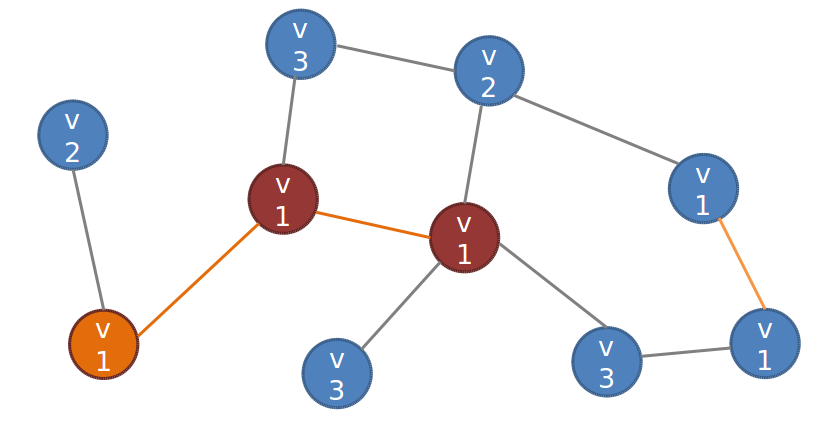
\includegraphics[width=1.0\linewidth]{Paul/python/graph.png}
     \caption{Représentation du système par un graphe}
     \label{graph}
\end{figure}

La première étape consiste à définir la répartition des logiciels dans le système. Afin de faire varier l'entropie, on utilise une distribution de Dirichlet. Celle-ci permet de s'approcher d'une distribution uniforme (proportions proches de $\frac{1}{n}$, grande entropie) ou au contraire de s'en éloigner (une proportion proche de 1 et les autres proches de 0, faible entropie). 

\begin{figure}[!ht]
\centering
     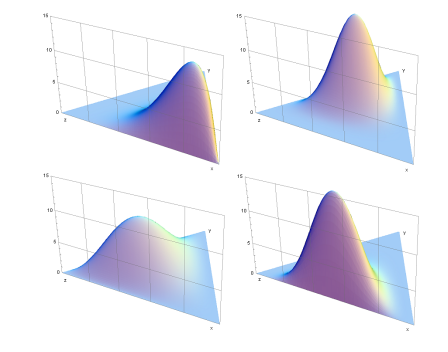
\includegraphics[width=1.0\linewidth]{Paul/python/dirichlet.png}
     \caption{Distribution de Dirichlet (source: Wikipedia)}
     \label{dirichlet}
\end{figure}

On répartit ensuite les logiciels au différents nœuds de manière aléatoire dans les proportions présentées précédemment.
Pour chacun des logiciels du système, on prend aléatoirement l'un des nœuds sur lequel il est présent comme le point d'entrée de l'infection. Les liens du graphe sont alors confirmés si chaque paire de nœuds correspondante est de cette version. Il nous suffit alors de compter le nombre de machines que l'on peut atteindre depuis la machine infectée initialement. Cela représentera l'ensemble des machines infectées du système si l'attaque vise cette version.
On somme alors les cardinaux de tous ces ensembles, pondérés par la proportion de la version du logiciel correspondante dans le système.
On effectue cette simulation cent fois de suite pour chaque distribution, et la moyenne des résultats nous donne l'étendue moyenne de l'infection en nombre de machines infectées, pour l'entropie correspondante.

Les résultats que l'on obtient sont présentés aux figures \ref{lfixe} et \ref{nfixe}, toujours pour 100 machines.

\begin{figure}[!ht]
\centering
     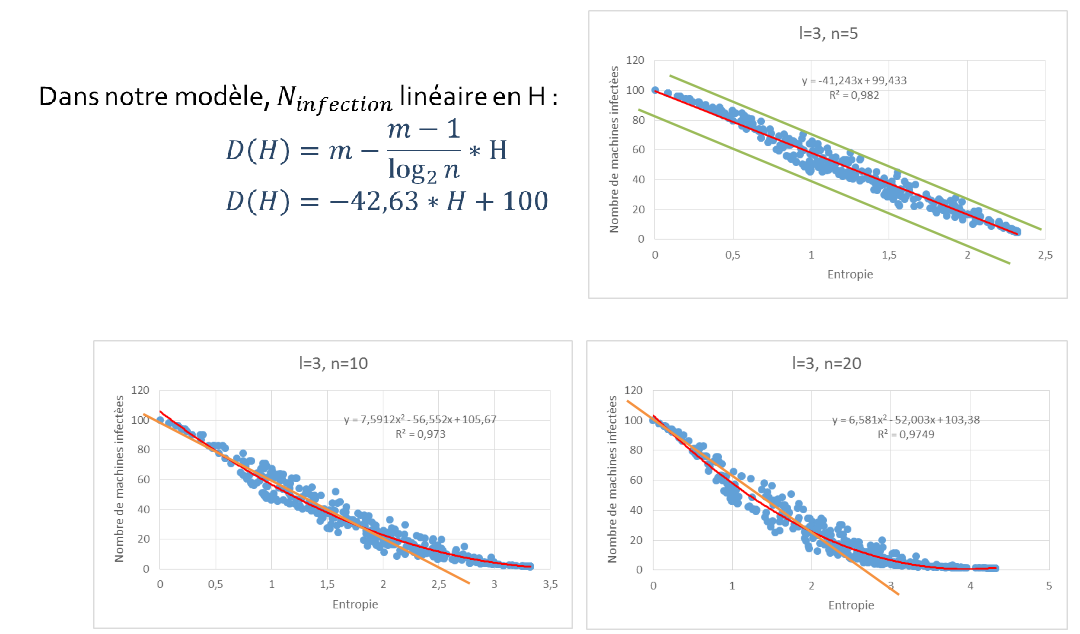
\includegraphics[width=1.0\linewidth]{Paul/python/lfixe.png}
     \caption{Simulation pour l fixé}
     \label{lfixe}
\end{figure}

Sur la figure \ref{lfixe}, on a fixé l (le degré de liaison entre les machines), mais on a fait varier n, le nombre de versions différentes dans le système. Un premier point intéressant à remarquer est qu'il y a bien une relation entre entropie et nombre de machines infectées. Pour $l=3$ et $n=5$, la relation est même linéaire. En effectuant une régression linéaire, on obtient une droite avec des coefficients très proches de ceux obtenus avec notre modèle présenté précédemment. Celui-ci est donc cohérent dans ce cas précis.
En faisant augmenter n, on constate cependant que la décroissance du nombres de machines infectées en fonction de l'entropie se fait plutôt de manière quadratique. Mais en se restreignant à des des valeurs entropies pas trop élevées (jusqu'à 2.5, ce qui sera rarement dépassé dans la réalité, cela correspondrait à quasiment installer une version différente sur chaque machine, ce qui est peu envisageable), on retrouve une bonne approximation linéaire. On peut donc en déduire que l'on peut étendre notre modèle à un nombre plus élevé de versions de logiciels, en n'augmentant pas trop l'entropie puisque de toute façon, cela a un intérêt de plus en plus réduit si elle devient trop élevée (la décroissance est alors beaucoup plus faible). Nous pouvons retenir de cette simulation que le nombre de versions des logiciels à une influence importante sur le nombre de machines infectées.


\begin{figure}[!ht]
\centering
     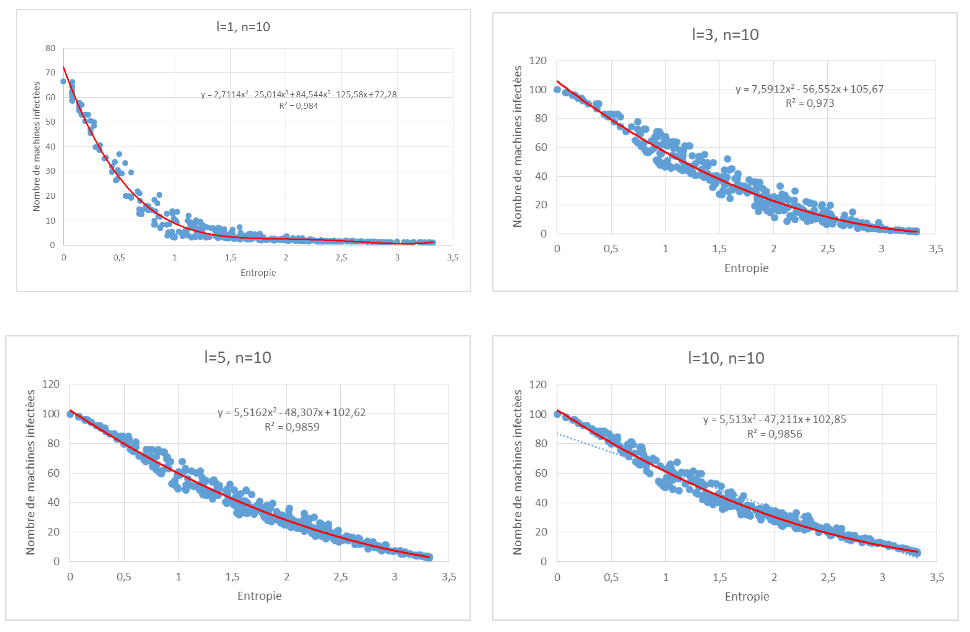
\includegraphics[width=1.0\linewidth]{Paul/python/nfixe.png}
     \caption{Simulation pour n fixé}
     \label{nfixe}
\end{figure}

Sur la figure \ref{nfixe}, on s'est intéresser à l'influence du nombre de liaisons, nous avons donc fixé le nombre de versions n et nous avons fait varier le degré de liaisons l. On remarque que pour des petites valeurs l, le faible nombre de liens réseau entre les machines contribue grandement à freiner la propagation du \textit{malware}. Même si nous sommes éloigné de notre approximation linéaire, nous pouvons nous contenter d'une faible entropie pour avoir une bonne défense, la faible valeur de l'entropie permettant d'avoir réduire l'infection du système. À partir de $l=5$ (cette valeur est relative à la taille du système en nombre m de machines), les résultats se stabilisent : il y a déjà assez de liens réseau pour que le \textit{malware} puisse se propager rapidement. L'entropie dans ce cas là est le facteur important comme moyen de défense, nous avons une décroissance très importante avec l'entropie, et l'on retrouve notre approximation linéaire.
Ce seconde type de simulation nous permet de voir que l n’a a priori qu’un impact relatif sur le nombre de machines infectées.

